%% ----------------------------------------------------------------
%% Thesis.tex -- MAIN FILE (the one that you compile with LaTeX)
%% ----------------------------------------------------------------

% Set up the document
\documentclass[12pt,a4paper,oneside]{csedu}  % Use the "Thesis" style, based on the ECS Thesis style by Steve Gunn
\graphicspath{{Figures/}}  % Location of the graphics files (set up for graphics to be in PDF format)

% Include any extra LaTeX packages required
\usepackage{graphicx}
\usepackage[square, numbers, comma, sort&compress]{natbib}  % Use the "Natbib" style for the references in the Bibliography
\usepackage{verbatim}  % Needed for the "comment" environment to make LaTeX comments
\usepackage{vector}  % Allows "\bvec{}" and "\buvec{}" for "blackboard" style bold vectors in maths
\hypersetup{urlcolor=black, colorlinks=true}  % Colours hyperlinks in blue, but this can be distracting if there are many links.
\usepackage{algorithm} % for writing pseducode
\usepackage{algorithm,algpseudocode}
\usepackage{amsthm}
\usepackage{array}
\usepackage{tabularx}

%% ----------------------------------------------------------------
\begin{document}
\frontmatter      % Begin Roman style (i, ii, iii, iv...) page numbering

% Set up the Title Page
\title{Sliding Window Based Infrequent Weighted Itemset Mining}
\authors  %{\texorpdfstring
         %{\href{your web site or email address}{Name}}
{Abdullah Al - Matin  \\Exam Roll: Curzon Hall-- 1085\\Registration No: EK - 895}
%{Your name should not appear on the external copies, write name between braces on the left}


%      {Author Name}
%   }
%\addresses  {\groupname\\\deptname\\\univname\\\FACULTY}  % Do not change this here, instead these must be set in the "Thesis.cls" file, please look through it instead, add roll, session and registration number ehich starts at line 204.
%\date       {\today}
%\subject    {}
%\keywords   {}

\maketitle

%% ----------------------------------------------------------------

\setstretch{1.5}  % It is better to have smaller font and larger line spacing than the other way round

% Define the page headers using the FancyHdr package and set up for one-sided printing
\fancyhead{}  % Clears all page headers and footers
\rhead{\thepage}  % Sets the right side header to show the page number
\lhead{}  % Clears the left side page header

\pagestyle{fancy}  % Finally, use the "fancy" page style to implement the FancyHdr headers

%% ----------------------------------------------------------------
% Declaration Page required for the Thesis, your institution may give you a different text to place here
\Declaration{

\addtocontents{toc}{\vspace{1em}}  % Add a gap in the Contents, for aesthetics

I, hereby, declare that the work presented in this project is the
outcome of the investigation performed by me under the supervision
of Dr. Chowdhury Farhan Ahmed, Associate Professor, Department of Computer
Science and engineering, University of Dhaka. I also declare that
no part of this project has been or is being submitted elsewhere
for the award of any degree or diploma.

\bigskip
\bigskip
\bigskip


%\begin{tabular}{lp{1in}r}
%\\ & \\ & \\


\begin{tabular}{c c c c}

  % after \\: \hline or \cline{col1-col2} \cline{col3-col4} ...
  Countersigned &\hspace{1.8in} & & Signature \\

   & & &  \\
  \ldots\ldots\ldots\ldots \ldots\ldots\ldots\ldots   & & & \ldots\ldots\ldots\ldots \ldots\ldots\ldots\ldots   \\
  (Dr. Chowdhury Farhan Ahmed) & & & (Abdullah Al - Matin) \\
  {\bf Supervisor} & & &  \\

 

\end{tabular}
}

\clearpage  % Declaration ended, now start a new page



% The Abstract Page
\addtotoc{Abstract}  % Add the "Abstract" page entry to the Contents
\abstract{
Now a days, frequent itemset mining is a popular approach. For finding frequent itemset, several approaches is already established. Infrequent items can be also very important for finding unexpected behavior like fraud detection, cost function minimization, equal task distribution for data center resource management etc. Weight may play a very important role in this scenario. In general approach, weighted itemset is treated all alike. But we have proposed an algorithm for mining infrequent weighted itemset by treating them differently based on their weight. Experimental results and graphs are added for the support of our proposed algorithm’s efficiency and effectiveness.
\addtocontents{toc}{\vspace{1em}}  % Add a gap in the Contents, for aesthetics

 }

\clearpage  % Abstract ended, start a new page
%% ----------------------------------------------------------------

\setstretch{1.3}  % Reset the line-spacing to 1.3 for body text (if it has changed)

% The Acknowledgements page, for thanking everyone
\acknowledgements{
\addtocontents{toc}{\vspace{.5em}}  % Add a gap in the Contents, for aesthetics
%
%
First of all, I am thankful and expressing my gratefulness to Almighty Allah who offers me His divine blessings, patient, mental and psychical strength to complete this project work.
%
I am deeply indebted to my project supervisor Dr. Chowdhury Farhan Ahmed, Associate Professor, Department of Computer Science and
Engineering, University of Dhaka. His scholarly guidance,
important suggestions, endless patience, constant supervision,
valuable criticism, and enormous amount of work for going through
my drafts and correcting them, and generating courage from the
beginning to the end of the research work has made the completion
of the project possible.\\
%
I would like to express my deep gratitude to Md. Samiullah
and Muhammed Tawfiqul Islam, lecturer, Dept of CSE DU for his
support and help for my work. The discussions with him on various
topics related my works have helped me to enrich my knowledge
and conception regarding this work.\\
%
Last but not the least; I am highly grateful to my parents and
family members for their support and constant encouragement, which
have always been a source of great inspiration for me.
}
\clearpage  % End of the Acknowledgements
%% ----------------------------------------------------------------

\pagestyle{fancy}  %The page style headers have been "empty" all this time, now use the "fancy" headers as defined before to bring them back


%% ----------------------------------------------------------------
\lhead{\emph{Contents}}  % Set the left side page header to "Contents"
\tableofcontents  % Write out the Table of Contents

%% ----------------------------------------------------------------
\lhead{\emph{List of Figures}}  % Set the left side page header to "List if Figures"
\listoffigures  % Write out the List of Figures

%% ----------------------------------------------------------------
\lhead{\emph{List of Tables}}  % Set the left side page header to "List of Tables"
\listoftables  % Write out the List of Tables

%% ----------------------------------------------------------------
\setstretch{1.5}  % Set the line spacing to 1.5, this makes the following tables easier to read
\clearpage  % Start a new page
%\lhead{\emph{Abbreviations}}  % Set the left side page header to "Abbreviations"
%\listofsymbols{ll}  % Include a list of Abbreviations (a table of two columns)
%{
% \textbf{Acronym} & \textbf{W}hat (it) \textbf{S}tands \textbf{F}or \\
%\textbf{LAH} & \textbf{L}ist \textbf{A}bbreviations \textbf{H}ere \\

%\textbf{} & \textbf{} \textbf{} \textbf{} \\
%}

%% ----------------------------------------------------------------
\clearpage  % Start a new page


\setstretch{1.5}  % Return the line spacing back to 1.3

\pagestyle{empty}  % Page style needs to be empty for this page
%\dedicatory{For/Dedicated to/To my\ldots}

\addtocontents{toc}{\vspace{2em}}  % Add a gap in the Contents, for aesthetics


%% ----------------------------------------------------------------
\mainmatter   % Begin normal, numeric (1,2,3...) page numbering
\pagestyle{fancy}  % Return the page headers back to the "fancy" style

% Include the chapters of the thesis, as separate files
% Just uncomment the lines as you write the chapters

% Chapter 1
\chapter{Introduction}
% Write in your own chapter title\label{Chapter 1}
\lhead{Chapter 1. \emph{Introduction}}
 % Write in your own chapter title to set the page header
%\section{Data mining}
 %
Data mining is the process for finding interesting and useful patterns from a dataset. The very first approach was finding frequent items i.e. the items that are used frequently. It plays an important role for finding knowledge discovery technique such as association rule mining, classification, clustering, time-series mining, graph mining, web mining etc. A lots of research and algorithm have been proposed for finding frequent patterns using Apriori based algorithms, FP tree based algorithms and others algorithms. In real life, frequent item set finding application is used in market basket analysis [], medical image processing [], biological data analysis [] etc. Traditionally, all items in a transaction are treated equally. Though all items interest/influence is not same, they should be treated differently. For solving this problem, the notion of weighted item set mining has been introduced []. The weight of an item is the value that signifies the local interest within each transaction. 
\par
Several approaches have been proposed for IWIM (Infrequent Weighted Itemset Mining). In those approaches, they consider all data from the very beginning of the database. Therefore these approaches cannot be applicable for a large-scale data set such as data streams [] where data set flows in the form of continuous stream. Data stream is a continuous, unbound and ordered sequence of items that comes in order of time. In this case, it is impossible to maintain all data from the dataset and cannot possible to process all data at a time.  
\par
Existing algorithm works on whole fixed dataset and generates infrequent item set. For data stream, it have handle data in an efficient manner. Older data will be lost and also new updated data have to process. So it should differentiate recently generated data from older information which may unimportant or obsolete in context of time.
\par
Consider as an example, the data set in Table~\ref{tab:Table} where there is a set of transactions from data stream. Here we have considered a small part of the data set for simplicity. It contains eight transactions. These transactions are identified by tids. Each transaction contains four distinct items with their weights. It’s not necessary to be exact four items. Weight is defined by the corresponding degree of interest in the transaction i.e. item {\it b} contains weight 43 in tid 2 but in tid 3 is 0. Item weight is the value of CPU usage readings at a specific time. For data stream this CPU usage reading is done at a fixed sampling rate. This CPU usage is important for data center resource management and application specific profiling. In tid4, weight of item {\it a} is 100. It means CPU a is working at high usage rate. While in tid 1, its weight is 0. It means temporarily {\it a} is idle. Knowledge extracting from this data set is important for domain expert or specific application expert to allocate system task break down for all CPU at a specific time.  So that, the system output can be maximized.
%

\begin{table}
\begin{center}
\begin{tabular}{ |c|c| } 
\hline
Transaction IDs (tid) & CPU usage reading \\
\hline
1 & (a,0) (b,100) (c,57) (d,71)\\
2 & (a,0) (b,43) (c,29) (d,71)\\
3 & (a,43) (b,0) (c,43) (d,43)\\
4 & (a,100) (b,0) (c,43) (d,100)\\
5 & (a,86) (b,71) (c,57) (d,71)\\
6 & (a,57) (b,71) (c,0) (d,71)\\
7 & (a,91) (b,32) (c,11) (d,0)\\
8 & (a,17) (b,61) (c,0) (d,72)\\
\hline
\end{tabular}
\caption{Example of a transaction data stream with weight}
\label{tab:Table}
\end{center}
\end{table}





%\begin{figure}[ht]
%\centering
%\includegraphics {transactions.eps}
%\caption{Transaction}
%\label{fig:trans}
%\end{figure}
%


%
%


\section{Basic Concepts}
 %
 This section will be updated later.
 \iffalse
The main approaches of data mining include:\\
\textbf{Frequent pattern, association and correlation mining:}
Frequent patterns are patterns that frequently occur in data. There are many kinds of frequent patterns, including itemsets, subsequences, and substructures. For example, if milk and bread are frequently bought items in a market, then $\{milk, bread\}$ is a frequent itemset. 
Association rule mining finds interesting relationships among a large set of data items. The association rules are considered interesting if they satisfy both a minimum support threshold and a minimum confidence threshold \cite{book}.
Correlation analysis is a measure which finds the underlying dependencies between itemsets of data.\\
%
\textbf{Classification:}
Classification is the problem of identifying to which of a set of categories a new data belongs. It is done on the basis of a training set of data whose class label is known.\\
%
\textbf{Cluster Analysis:}
Cluster analysis deals with data for which the class labels are not known. Here, data is clustered or grouped based on the principle of maximizing the intraclass similarity and minimizing the interclass similarity \cite{book}. \\
%
\textbf{Outlier Analysis:}
A data set may contain some data which behaves differently than the rest of the data. This type of data is known as outlier. Sometimes this outliers provides us with useful information about the dataset. Analysis of these outlier data is known as outlier analysis.  
%
\section{Infrequent Itemset Mining} \label{sec:graph_mining}
%
Frequent itemset mining is a very common approach for finding frequent items. In our approach, we are trying to find infrequent items. Those  are the infrequent items, whose value is below threshold. For a given max{\_}support value, items value is below the max{\_}support. Infrequent item is important for resource management, application profiling, and fraud detection. It can be used for finding any unexpected or abnormal behaviour of a system. 

%
%\begin{figure}[ht]
%\centering
%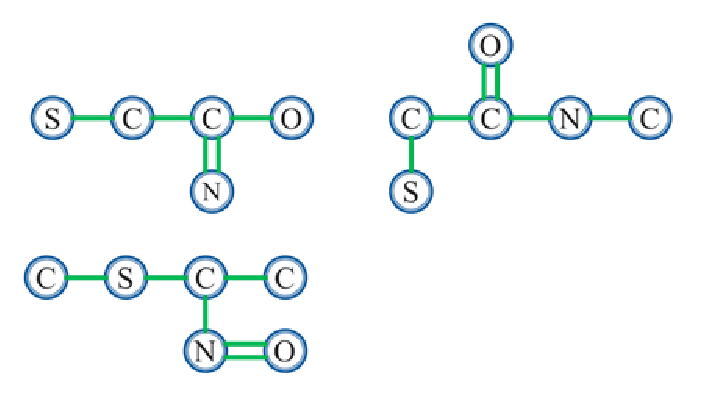
\includegraphics[scale = 0.8] {graph_data.eps}
%\caption{a set of chemical compounds represented using graph}
%\label{fig:graphdata}
%\end{figure} 
%
%
\fi


\section{Motivation}
%
Mining for infrequent itemset is recently gained attention of research community. Main focus for finding infrequent itemset whose frequency value is below \texttt{max\_support}. Not only frequency, weight can be also used for finding infrequent itemset mining. \\

\par
Let’s consider a scenario. A banking system where lots of transactions is done every day. As a bank officer, one may want to know if everything okay or not. In general cases, all transactions are okay but in fraud cases or unexpected cases, it may vary. It’s difficult for a bank officer to browse all data of the transactions to find any abnormal cases every day. It’s pretty hard for him. \\
\iffalse
%
\par \textbf{Motivating scenario:} \\
An application domain of graph classification related to the context of Bangladesh is drug discovery. Drug design and discovery is a growing field of interest in Bangladesh. The goal in drug discovery is to analyze this huge chemical space and identify molecules that show a certain desired activity. However, given the magnitude of the chemical space, an exhaustive exploration is not feasible \cite{drug}. Graph classification can be effectively used in this domain for molecular classification. \\
%
%\par The main goal of a graph classification approach is to classify graphs accurately and efficiently. But if we see some of the existing works we will find that, \\
%

\begin{itemize}
\item GAIA \cite{gaia} is a graph classification approach that makes use of evolutionary computation for feature selection purpose. But, it selects features by assigning  a score to a subgraph by only considering its own occurrence in the positive/negative graphs, it does not consider any other parameters. For this reason, its performance in terms of accuracy is not sufficient.
%
\item D\&D \cite{dnd} is one of the latest works in the field of graph classification. It provides a diversified discriminative score based on edge cover probability to select features. However, its performance is still not at satisfactory level. There is scope of improvement in terms of accuracy and runtime.
\end{itemize}
%
The above mentioned lackings of the existing works motivate us to develop a better graph classification approach.
%
\fi
\section{Objective}
%
We have studied that the existing approaches are limited to some context. As a solution, we have to develop an algorithm that can overcome the limitations. The objectives of our work are listed below:
%
\begin{itemize}
\item To carry out an extensive literature view regarding the infrequent itemset mining approach.
\item Propose a new efficient algorithm for finding infrequent items. 
\item Propose an algorithm that can perform in broader area.
\end{itemize}
%
\section{Thesis Contribution}
%
The contributions our research work are listed below:
%
\begin{itemize}
%
\item We have used sliding window based approach. This reduces the processing time \& memory space.
%
\item We can get the actual contribution of an item in the dataset. Previous approach uses equivalence weighting function for data items.
% 
\item It’s easier to discard frequent items from the candidate infrequent pattern list.
\item Extra cost for checking infrequent patterns validation (i.e. is the item actually infrequent or not) is not required.
%
\end{itemize}
%
\section{Thesis Outline}
The five chapters labeled as Introduction, Related Work, Proposed Approach, Performance Evaluation and Conclusion form the shape of the book.
Every chapter comprises of the following topics: \\
%
Chapter 1 contains some introductory concepts such as data mining and various data mining approaches, infrequent itemset mining and also the motivation and contribution of this work.\\
%
Chapter 2 describes various terms related to previous work in the field of infrequent itemset mining and also the limitations of the existing approaches. \\
%
Chapter 3 describes the proposed score and algorithm. It also contains the details of our work and application of the proposed algorithm. \\
%
Chapter 4 contains the implementation results and performance evaluation results of the proposed algorithm. \\
%
Chapter 5 draws the conclusion of the thesis by summarizing the
findings in the thesis and describing scope of possible extensions to this work. \\
%
The last part of the book is Bibliography which places all the reference cited in the work. The appendix works as additional information that helps the reader if necessary.
%
 % Introduction



 \chapter{Previous Work} % THIS COMMAND MAKES A SECTION TITLE.
 \label{Chapter 2}
 \lhead{Chapter 2. \emph{Previous Work}}
 This section will be added later.
 
 \iffalse
%
In this chapter, we discuss some basic terminologies and background knowledge in graph mining. We also discuss some recent works in the field of graph mining and graph classification. Here, we highlight their working procedure and analyze the algorithms.
% and also provide examples for better understanding of the algorithms.
 We also include the terminologies needed to understand the approaches. 
%
\newtheoremstyle{remboldstyle}
  {}{}{}{}{\bfseries}{.}{.5em}{{\thmname{#1 }}{\thmnumber{#2}}{\thmnote{ (#3)}}}
\theoremstyle{remboldstyle}
\newtheorem{defn}{Definition}
%
\section{Graph mining}
%
In section \ref{sec:graph_mining} of chapter 1, we have discussed about graph mining. Here we provide some basic terminologies in graph mining, which are needed to understand the following sections.
%
\begin{defn}[Graph having Labels]
Given a set of vertices $V(G) = \{v_1, v_2,---, v_k\}$, a set of edges connecting some vertex pairs in $ V(G), E(G) = \{ e_h = (vi, vj) \mid vi, vj \in V (G)\} $, a set of vertex labels $ L(V (G)) = \{lb(vi) \mid \forall vi \in V(G)\} $ and a set of edge labels $L(E(G)) = \{lb(e_h) \mid \forall e_h \in E(G)\} $, then a graph G is represented as $ G = (V (G),E(G), L(V (G)), L(E(G)) ) $.
\end{defn}
%
\begin{defn}[Size of a Graph]
The $size\ of\ a\ graph$ G is usually defined by the number of vertices or number of edges of the graph.
\end{defn}
%
\begin{defn}[ Graph Transaction and Graph Dataset]
A graph G = (V(G), E(G), L(V(G)), L(E(G))) is a $transaction$, and $graph\ dataset$ $GD$ is a set of transactions, where GD = $ \{ G_1,G_2,---,G_n \}$
\end{defn}
%
\begin{defn}[Support and Confidence]
Given a graph $G_s$, the $support$ of $G_s$ is defined as\\
$sup(G_s) = \dfrac
{number\ of\ graph\ transactions\ G\ where\ G_s \subset G \in GD}
{total\ number\ of\ graph\ transactions\ G \in GD }$
\\ \\
Given two subgraphs $G_b$ and $G_h$, the $confidence$ of the association rule
$G_b \Rightarrow G_h$ is defined as \\
$conf(Gb \Rightarrow Gh) = \dfrac
{number\ of\ graphs\ G\ where\ G_b \cup G_h \subset G \in GD}
{number\ of\ graphs\ G\ where\ G_b \subset G \in GD}$ \\
\end{defn}
%
\begin{defn}[Isomorphism and Subgraph Isomorphism]
An $isomorphism$ is a function $f:V(G) \rightarrow V(G')$, such that 
$ \forall u \in V(G), l_G(u)=l_G'(f(u)) $, and
$ \forall (u,v) \in E(G), (f(u),f(v)) \in E(G')$ and $l_G(u,v)=l_G'(f(u),f(v))$
%
A $subgraph\ iso- morphism$ from G to G' is an isomorphism from G to a subgraph of G'.
\end{defn}
%
\begin{defn}[Frequent Subgraph and Frequent Subgraph Mining]
Given a graph dataset $GD = \{G_1,G_2,---,G_n\}$, and a minimum support threshold $minSup$, let\\
%
$ \alpha(g,G)$ = \Bigg \{ \begin{tabular}{l}
1 if g is isomorphic to a subgraph of G,\\
0 if g is not isomorphic to any subgraph of G\\
\end{tabular}
\\
%
Then,\\
\centerline { $ \sigma(g,GS) = \Sigma_{G_i \in GS}\ \alpha(g,G_i)$}\\
where $\sigma(g,GS)$ denotes the frequency of g in GS.\\
Here, g is called a $frequent\ subgraph$ if its frequency is greater than or equal to $minSup$.
$Frequent\ subgraph\ mining$ is to find every graph g, such that $\sigma(g,GS)$ is greater than or equal to $minSup$.
\end{defn}
%
\begin{defn}[Embedding]
Given two graphs f and g, suppose $f \subseteq g$ by a subgraph isomorphic function $\alpha$. The subset of vertices of $V(g), V(g)_{\alpha} = \{ \alpha(u)|u �\in V(f) \}$, is a vertex embedding of f in g. In a similar way, the subset of edges of $E(g), E(g)_{\alpha} = \{(\alpha(v), \alpha(u))|(v, u) \in E(f)\}$ is an edge embedding of f in g.
\end{defn}
%
%
%\subsubsection{FSG}
%
%\subsection{gSpan}
%
\section{Graph Classification}
%
\subsection{GAIA}
%
\textbf{[GAIA: Graph Classification Using Evolutionary Computation]}\\
In the paper \cite{gaia}, the authors have proposed an algorithm for performing classification of graphs in a graph dataset.
\par The key features of gaia are the following:
\begin{itemize}
\item It proposes a subgraph encoding method using the notion of conditional canonical adjacency matrix.
\item It proposes a feature selection method that applies evolutionary computation.
\end{itemize}
%
\subsubsection{Terminologies}
%
\begin{defn}[Embedding code]
Given a subgraph isomorphism $f: V(g) \to V(g')$, the node set $\{f(u) | u \in V(g)\}$ is a vertex embedding of g in g'. A sorted embedding organizes the nodes in an vertex embedding in increasing order of their node IDs. An $embedding\ code$ B is the concatenation of the graph ID of g' and the sorted embedding. The first element in an embedding code is the graph ID and the remaining elements are node IDs.
\end{defn}
%
\begin {defn}[Adjacency matrix]
Given an embedding code B of pattern p based on a subgraph isomorphism f, the adjacency matrix M of p is a $\mid V \mid \times \mid V \mid $ matrix, where V is the node set of pattern p and each entry of M satisfies:\\
%
  M[i,j]=  \Bigg \{ \begin{tabular}{c}
label(B[i]) if i = j, or \\
label(B[i],B[j]) if $i \ne j$ \\
\end{tabular} 


         
%
\end {defn}
%
\begin {defn}[matrix code]
The matrix code of a subgraph pattern p is the sequence formed by row-wise concatenation of the lower triangle entries of an adjacency matrix M of p.
\end {defn}
%
\begin {defn}[Conditional Canonical Adjacency Matrix]
Conditional canonical adjacency matrix of a subgraph pattern p is the adjacency matrix corresponding to the lexicographically smallest embedding code of p.
\end {defn}
%
\begin {defn}[CCAM code]
It is the matrix code corresponding to the conditional canonical adjacency matrix of p.
\end {defn}
%
\subsubsection{Subgraph encoding method}
%
The computation is completed in three steps:
\begin{itemize}
\item Retrieve embeddings with the smallest graph ID.
\item For each embedding, sort the node IDs in ascending order and keep track of the lexicographically smallest embedding code B.
\item Construct the conditional canonical adjacency matrix according to B and generate the CCAM code.
\end{itemize}
%
\subsubsection{Fitness function}
%
\begin {defn}[Positive frequency]
Positive frequency of a subgraph pattern p, \\ \\
$(r^+(p)) =\dfrac{ number\ of\ positive\ graphs\ containing\ p}{ total\ number\ of\ positive\ graphs\ in\ the\ database}$ \\
\end {defn}
%
\begin {defn}[Negative frequency]
Negative frequency of a subgraph pattern p, \\ \\
$(r^-(p)) =\dfrac{ number\ of\ negative\ graphs\ containing\ p}{ total\ number\ of\ negative\ graphs\ in\ the\ database}$
\end {defn}
%
\begin{defn}[Log Ratio Score]
$log\ ratio\ score\ of\ pattern\ p = log \dfrac{r^+(p)}{r^+(p)}$
\end{defn}
%
\begin{defn}[Score Per Edge]
$score\ per\ edge\ of\ pattern\ p = \dfrac {log \dfrac{r^+(p)}{r^+(p)} } {m(p)}$ \\
Where, m(p) = number of edges in p
\end{defn}
%
\subsubsection{Framework of the pattern evolution}
For each graph $g_i$ in the positive graph set $G^+$, a representative subgraph pattern and a list of up to s candidate subgraph patterns is stored. Only subgraphs of $g_i$ with positive log ratio scores can be its representative or in its candidate list. The representative pattern has the highest log ratio score among all patterns that are subgraphs of gi and found during pattern evolution. Although one pattern can be subgraphs of several positive graphs, each pattern can only be in one candidate list at any time. The candidate lists are initialized with one-edge patterns.
The total number of subgraph patterns that the candidate lists can hold at any time is the product of s and $\mid G+ \mid$, Motivation behind this is to cause selection pressure to speed up the convergence of evolutionary search.
%
\subsubsection{Pattern extension}
Probability of pattern p in candidate list of $g_i$ to be selected for extension is: \\ \\
$ \dfrac{log\ ratio\ score\ (p)}{\Sigma _{p'\ is\ in\ the\ candidate\ list\ of\ g_i\ } log\ ratio\ score(p')}$ \\
\par The intuition here is that candidate patterns with higher scores are more likely to be extended to patterns with high scores. \\
%
To perform pattern evolution, GAIA runs for n iterations, where n is a parameter set by the user. During each iteration, one pattern is selected from each candidate list for extension. For an extension operation of pattern p, GAIA generates a pattern set X(p) and each pattern p' in X(p) has one new edge attached to p. A lookup table is used to determine whether a pattern has already been generated to avoid repetitive examination of the same pattern. \\
%
If pattern p extends into pattern p' and the log ratio score of p' is less than that of p, p' is eliminated from survival and further extension. If the score per edge function decreases steadily during successive extensions, these extensions are also pruned. 
%
\subsubsection{Pattern migration and competition}
%
A pattern that has already been extended are removed from the candidate lists. Some pattern in the candidate list may migrate to the candidate list of another graph if such migration will increase its chance of survival. Let p be the candidate pattern for migration and G(p) be the set of graphs containing p and $g_i$ be the graph in G(p) which has the lowest value of \\ 
%
${\Sigma _{p'\ is\ in\ the\ candidate\ list\ of\ g_i\ } log\ ratio\ score(p')}$ 
%
\par p will migrate to the candidate list of $g_i$. If the candidate list of $g_i$ has vacant positions, then p can move into one vacant position directly. If the candidate list is already full, then p has to compete with the "resident" patterns in the list. The score of p is compared against the score of a pattern p', which is randomly selected with probability 1/s from the candidate list. If the score of p is higher, then p' is eliminated and p takes the position of p', otherwise, p is eliminated.
%
\subsubsection{Generating association rules}
Association rule is defined as a classification rule A in the form of $p\to L$, where p is a subgraph pattern and L is the class label. If an object has the subgraph pattern p, then it is classified as L. The output of GAIA is an association rule set A. The accuracy of the association rule set A is calculated as follows:\\ \\
$Sensitivity\ = \dfrac{number\ of\ prediction\ that\ are\ positive\ and\ correct}{number\ of\ graphs\ that\ are\ positive}$ \\ \\
%
$Specificity\ = \dfrac{number\ of\ prediction\ that\ are\ negative\ and\ correct}{number\ of\ graphs\ that\ are\ negative}$ \\ \\
%
$Normalized\ accuracy\ = \dfrac{sensitivity + specificity}{2}$ \\ \\
%
\textbf {Association rule generation algorithm}
%
\begin{itemize}
\item The representative subgraph patterns are sorted by their log ratio scores in decreasing order 
\item	Then the representative patterns are traversed in the sorted order 
\item	For each representative pattern p
%
\begin{itemize}{
\item	Evaluate whether inclusion of a new association rule $p \to positive$ in the resulting association rule set A can increase the normalized accuracy
\item	The new rule $p \to positive$ is to be included in A if the normalized accuracy increases}
\end{itemize}
\item	The algorithm terminates when all representative patterns have been tested
\end{itemize}
%
\subsubsection{Analysis}
%
GAIA proposes a subgraph encoding method that uses embedding information. The complexity of the method is O(v2) , where v is the number of nodes in the pattern. It also proposes a feature selection method based on evolutionary computation approach.
\\
But while calculating the fitness function, it only considers its own occurrence in the positive/negative graphs. But it does not take any other parameter into consideration. There are various important parameters which can increase the performance of the feature selection method, if taken into account.
%
\subsection{D\&D}
%
\textbf{[Graph Classification: A Diversified Discriminative Feature Selection Approach]}\\
The authors of D\&D \cite{dnd} propose a graph classification model with a new score called diversified discriminative score. They highlight two issues with the existing feature selection approaches, namely:\\
%
\textbf{Highly overlapped features:}
%
The discriminative features selected can be possibly highly overlapped.
Two discriminative features, $f_i$ and $f_j$ , may share a large common part.
They may not lead to a good classification accuracy, because one of them is redundant in a sense that they appear frequently together in graphs in D. \\
%
\textbf{Missing Important Features:}
Some important features may be missed out as the number of discriminative features selected for building a classifier is often restricted.\\
% 
To remove these issues, they propose a approach which explores the additional value of the diversity together with the discriminativity. It also explores how to reduce the overlapping between a feature and a set of features, based on edge-cover.
%
\subsubsection{Terminologies}
%
\begin {defn}[Graph coverage]
Given a graph database $D = \{g_1, g_2,---, g_n \}$ and a feature f, a graph $g_i \in D$ is covered by f if, there is an edge embedding of f in $g_i$.
\end {defn}
%
\begin {defn}[Edge cover  $E_c ( f,g ) $]
It is the set of edges in g covered by feature f.
\end {defn}
%
\begin {defn}[Feature edge cover $C_e(f)$]
It is the set of edges that are covered by f in all graphs in D.\\
\centerline{$C_e(f) = \cup_{g_i \in sup(f)} E_c(f, g_i)$}
\end {defn}
%
\begin {defn}[Edge cover score $S_c ( f ) $]
It is the number of edges covered by f in all graphs in D.\\
\centerline{ $S_c(f) = \Sigma_{g_i \in sup(f)} |E_c(f, g_i)|$}
\end {defn}
%
\begin {defn}[Edge cover probability $P_c ( f ) $]
Edge-cover probability of a feature f regarding to
the entire edge set in D is,
$P_c(f) = \dfrac{|C_e(f)|}{ \Sigma _{g_i\in D} |E(g_i)|} $
\end {defn}
%
\subsubsection{Fitness Score}
%
In this paper, they propose a score that calculates the diversity of a discriminative subgraph. Diversity of a feature $f_{m}$ with respect to a set of selected features $F_{m-1}$ is,\\
%
$p_d(f_m) = p_c(F_m) - p_c(F_{m-1})$\\ \\
%
$ = \dfrac {\mid C_e(f_m) - C_e(f_m �\cap F_{m-1}) \mid }{\Sigma _{g_i \in D} \mid E(g_i) \mid} $ \\ \\
%
$ = \dfrac {\mid C_e(f_m) - \Sigma ^{m-1} _{j=1} C_e(f_m \cap f_j ) \mid}{\Sigma _{g_i \in D} \mid E(g_i) \mid}$ \\ \\
%
$= \dfrac {\Sigma _{g_i \in sup(f_m)} \mid E_c(f_m, g_i)\mid}{\Sigma _{g_i \in D} \mid E(g_i) \mid} -
\dfrac { \Sigma _{g_i \in sup(f_m)} \mid \cup^{m - 1} _{j=1} (E_c(f_m, g_i) �\cap E_c(f_j, g_i))\mid}{\Sigma _{g_i \in D} \mid E(g_i) \mid}$ \\ \\
%
Let,\\
$p^+ _d(f_m)$ = the diversity of $f_m$ for the set of positive graphs $(D^+)$,\\
% 
$p^- _d(f_m)$ = the diversity of $f_m$ for the set of negative graphs $(D^-)$ \\
%
Then the diversified discriminative score of feature $f_m$, \\ \\
\centerline{$score_d(f_m) = log\dfrac {p^{+} _{d} (f_m)}{p^{-}_{d} (f_m)}$}
%
\subsubsection{D\&D algorithm}
%
\begin{algorithm}
 \caption{D\&D (D,F,K)}
  Input: A graph database $D = (D^+, D^-)$,\\
             a set of frequent subgraphs F, \\
                the number of features, K\\
Output: a selected feature set $F_s$
\begin{algorithmic}[1]
 \State {$f \gets argmax _{f \in F} \ logRatioScore(f);$\\
 $Fs \gets {f};$}
\While {$|F_s| \le k$}

 \State $f \gets argmax _{f \in F/F_s} \ score_d(f);$
 \State $F_s \gets F_s \cup{f};$
\EndWhile	\\
\Return $F_s$;
\end{algorithmic}
 \end{algorithm}
%
\subsubsection{Analysis}
%
D\&D proposes a diversified discriminative score based on edge cover probability. The score reduces selection of discriminative subgraphs which are overlapped with each other.\\ 
Using this diversified discriminative score, they provide an algorithm that selects a number of discriminative subgraphs as features based on the score.  The complexity of the algorithm is O(K.F), where K = number of features to be selected in the feature selection phase and F = is the set of discriminative subgraph from which the features will be selected.\\
The accuracy of D\&D is still not satisfactory. There is scope of improvement in terms of accuracy which can be achieved by taking the proper parameters into account and incorporating them in the fitness score.
%
\section{Summary}
%\end{document} % THE INPUT FILE ENDS LIKE THIS
\fi % Previous Work

% Chapter 3
\chapter{Proposed Approach} % Write in your own chapter title
\label{Chapter 3}
\lhead{Chapter 3. \emph{Proposed Approach}} % Write in your own chapter title to set the page header
In this chapter we present our proposed scoring system for evaluating subgraphs. We also discuss the feature selection algorithm and classification algorithm which will use the proposed score to classify graphs. 
%\section{Introduction}
%
%\section{Terminologies}
%
%\section{Problem Definition and Solution Methodology}
%
\section{Problem Definition}
%
This paper address the problem of infrequent weighted itemset mining from a transaction dataset. Let {\it I} = \{{\it i1, i2. . . . . ,im}\} a set of data items. Transactional dataset {\it T} =\{{\it t1, t2, t3 . . . . . ,tn}\} is a set of transaction where each transaction is a set of items in {\it I} and denoted by transaction ID (tid). 

An Item set is a set of data items i.e. in {\it k} item sets there is {\it k} items.  Support for an item is the count of that item in the dataset. Based on support count, an item may be frequent or infrequent. For identify an item as frequent or infrequent, a threshold {\it E} is used. This threshold can be set based on user interest. In this paper, we are targeting infrequent items. So, we need to discard items that are above the threshold. 

In regular basis, for frequent item set mining, items and transactions are consider in the same way. But [Ref] according to this paper, we also treating each item differently. Here, each item is paired with it’s weight i.e ({\it I,k}), {\it I} is an item contain in the transaction set {\it T}, {\it K} is the weight of the item that signifies the interest/intensity in the transaction.

As we are working on data stream, we need to process data in an efficient manner. To find infrequent itemset mining from a data stream, we can’t perform multiple scan from a data stream. Once the streams flow  through we lose them. To find recent important knowledge from a data stream, Single-pass and sliding window based mechanism [] is required. 

We have adopted similar definitions presented in the previous works (Carter er al., 1997; Barbar and Hamilton, 2000, 2001, 2003; Li et al., 2005a,b). Let {\it I} = \{{\it i1, i2 . . . . . . , im}\} be a set of items and {\it D} be a transaction database \{{\it T1, T2 . . . . . . , Tn}\} where each transaction {\it Ti} ϵ {\it D} is a subset of {\it I}.
%Definition 1: The measure value mv(ip, Tq), represents the weight of an item ip in transaction Tq. For



%

%
\section{Solution Methodology}
%
In this section, We describe the construction process of our tree structure to store the stream data using a single pass. We use ShrFP-Tree (Share-frequent pattern tree) for share-infrequent pattern mining. The header table is maintained to keep an item order in our tree structure. Each entry of a transaction in a header table  explicitly maintains item-id and weight information for each item. Here, weight is the {\it tmv} (transaction measure value) values of items. To facilitate the tree traversals adjacent links are also maintained (not shown in figure for simplicity) in our tree structure.
%
\par Consider the example data stream at Table~\ref{tab:Table} . At first, ShrFP-Tree captures the {\it tmv} values of all items and keep in header table  as weight. After that, we scan each database transaction one by one and then insert in the tree. In our example, first transaction T1 contains four items one of which is 0. If any item’s weight is 0 in the transaction, we will not insert that item in the tree. So, now we have three transactions {\it b,c,d} and insert them in the tree. 
\begin{figure}[ht]
\centering
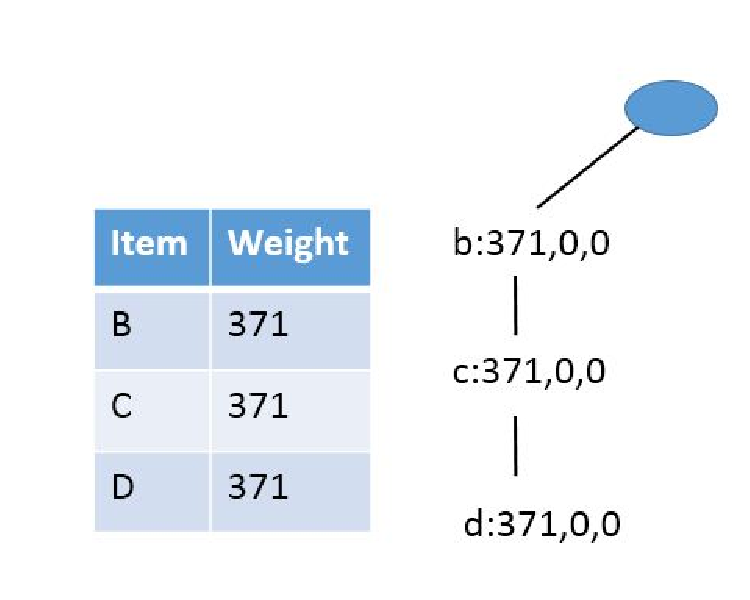
\includegraphics[scale = 0.8] {a.eps}
\caption{After inserting batch 1}
\label{fig:insert1}
\end{figure} 
Figure ~\ref{fig:insert1} shows the tree and header table after inserting batch 1. 
\begin{figure}[ht]
\centering
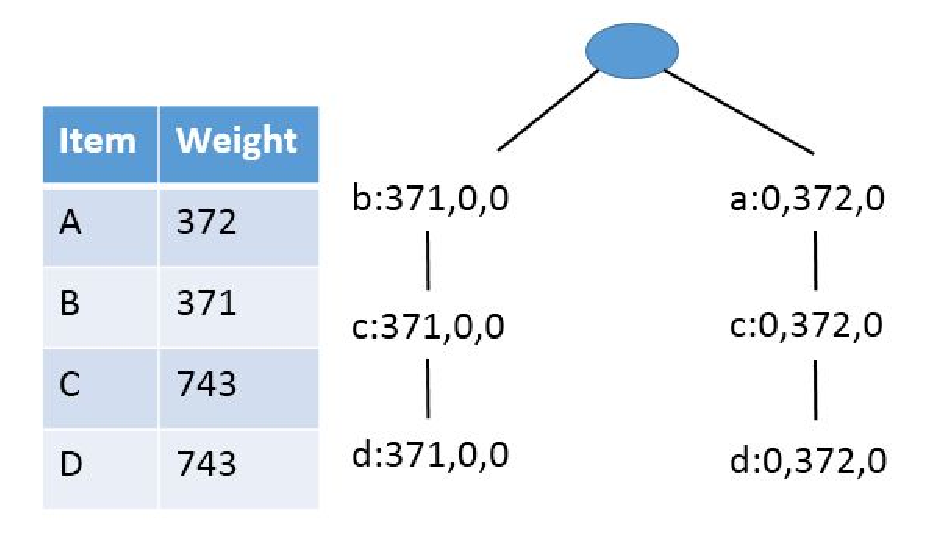
\includegraphics[scale = 0.8] {b.eps}
\caption{After inserting batch 2}
\label{fig:insert2}
\end{figure} 
\begin{figure}[ht]
\centering
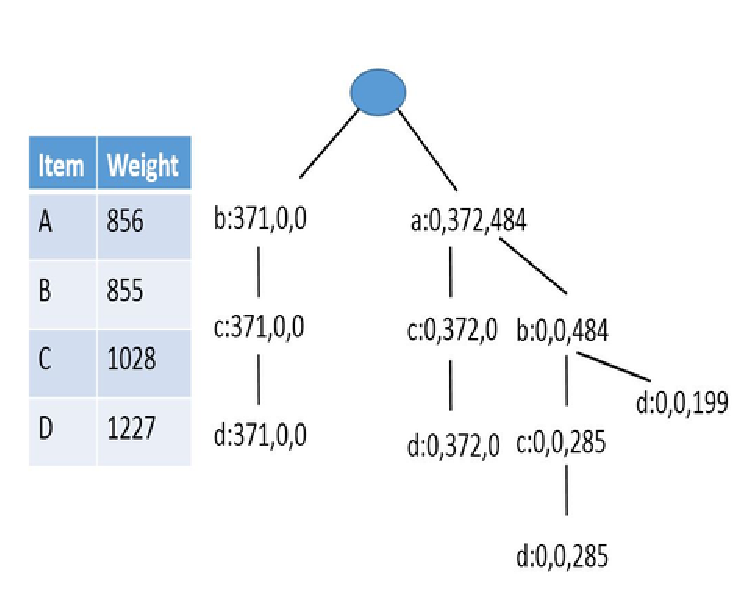
\includegraphics[scale = 0.8] {c.eps}
\caption{After inserting batch 3}
\label{fig:insert3}
\end{figure}
%
\begin{figure}[ht]
\centering
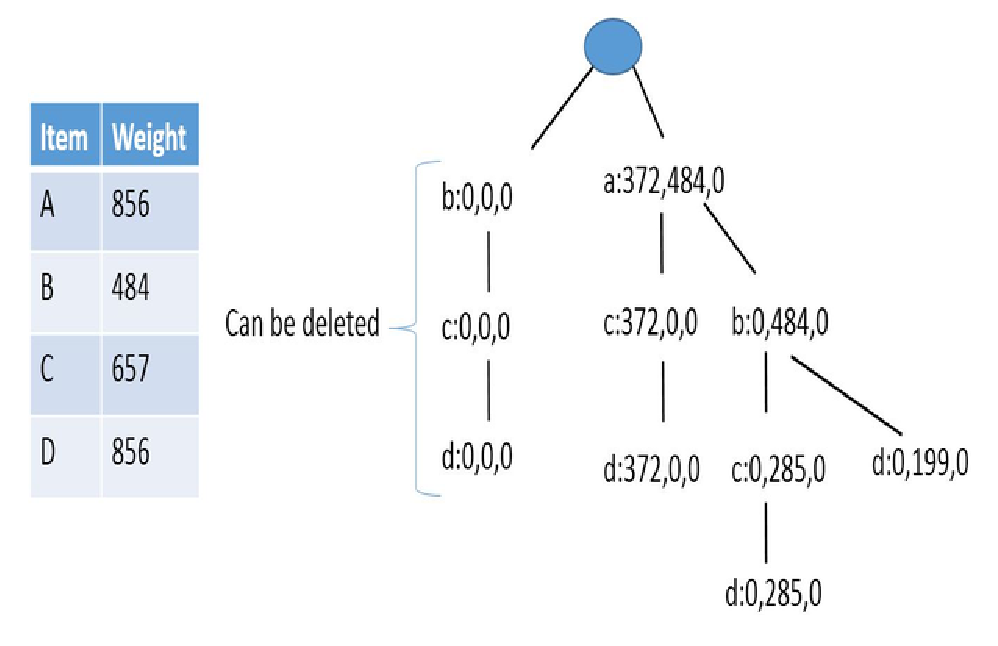
\includegraphics[scale = 0.8] {d.eps}
\caption{Deletion process of batch 1}
\label{fig:insert4}
\end{figure}


\begin{figure}[ht]
\centering
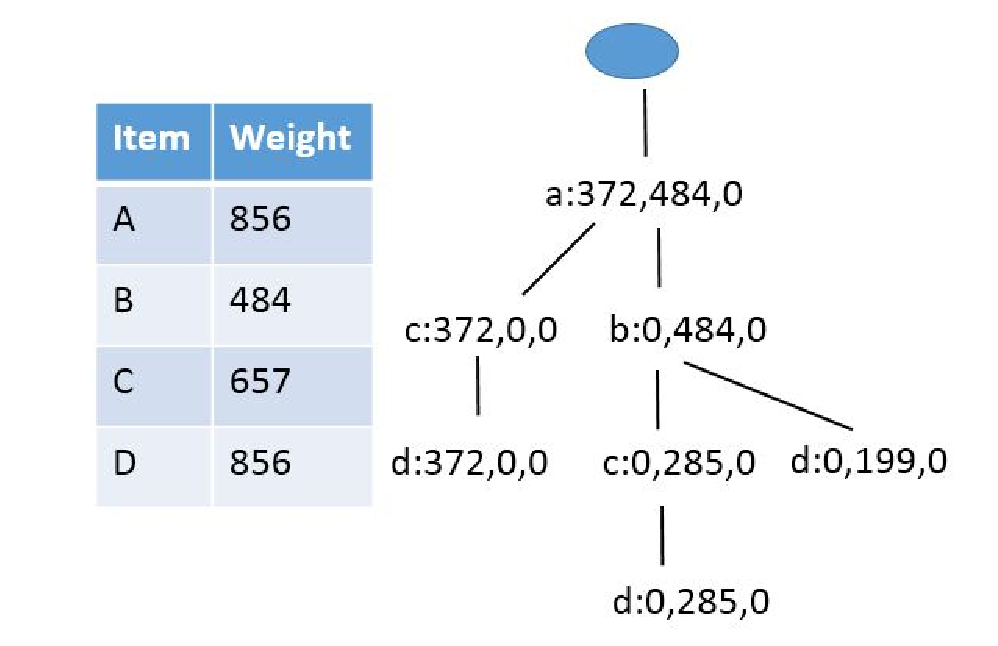
\includegraphics[scale = 0.8] {e.eps}
\caption{After deleting batch 1}
\label{fig:insert5}
\end{figure}


\begin{figure}[ht]
\centering
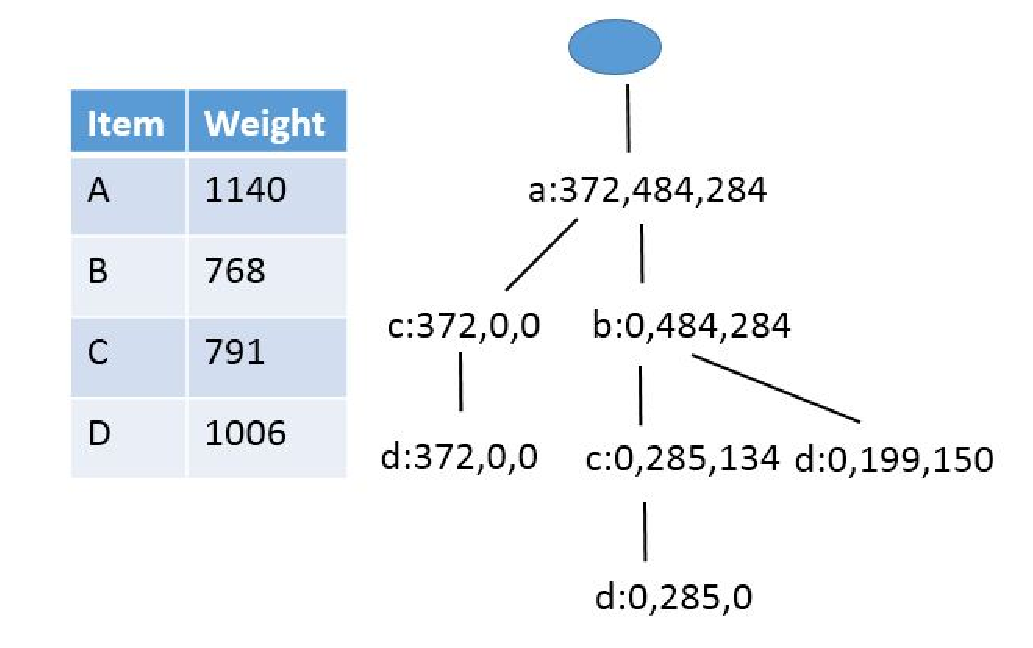
\includegraphics[scale = 0.8] {f.eps}
\caption{After inserting batch 4}
\label{fig:insert6}
\end{figure}
%

\begin{figure}[ht]
\centering
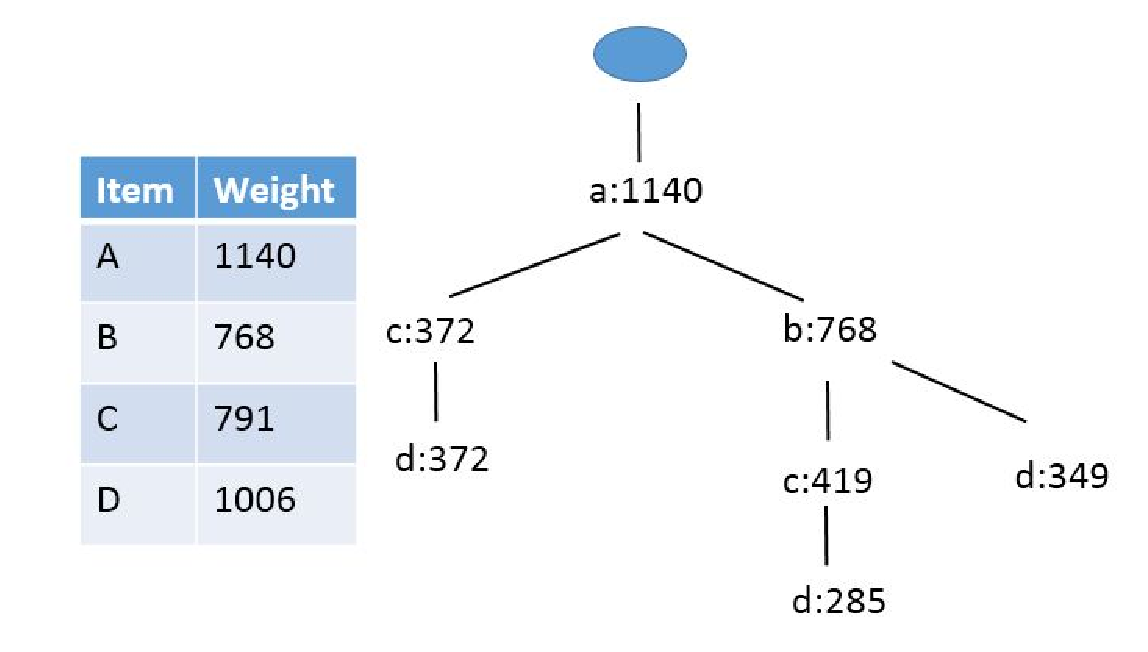
\includegraphics[scale = 0.8] {g.eps}
\caption{Complete tree after inserting window 2}
\label{fig:insert7}
\end{figure}

Figure ~\ref{fig:insert2} shows the tree and header table after inserting batch 2. In the same way, batch 3 also inserted in the tree. The final tree after inserting window 1 in the tree is shown in Figure ~\ref{fig:insert3}.

\par As it’s a data stream, the stream moves to batch 4. It needs to delete previous information of batch 1. Because batch 1 is not belongs to window 2 and therefore the information of batch 1 becomes garbage in the window 2 and it will no longer be used. We delete information of batch 1 from the tree. We also update the header table. After deletion of batch 1, the header table and the tree is shown in Figure ~\ref{fig:insert5}. Some nodes which do not have any information of batch 2 and batch 3. We can delete them from the tree. In case of other nodes, the weight are shifted one position left to remove the weight information of batch 1. Now insert new batch i.e. batch 4 in the tree. As a result, the three weight information of each node represents batch 2, batch 3 and batch 4. Figure ~\ref{fig:insert6} shows the tree after insertion of batch 4.
%
\\*
{\bf Property 1:} The total value of {\it tmv} (transaction measure value) of any node in ShrFP-Tree is greater than or equal to the sum of total value of {\it tmv} values of its children.
\clearpage
\section{Mining Process}
ShrFP-Tree is a pattern growth mining process that mines all the candidate share-infrequent patterns. According to our property 1, pattern growth mining algorithm can be directly applicable to it by using {\it tmv} values.
\par Consider the database of Table~\ref{tab:Table} and maxShare = 0.20 in that database. The final ShrFP-Tree for the database we have considered in Table~\ref{tab:Table}, is shown in Figure ~\ref{fig:insert7}. At first, we have prepared a header table for all items. According to header table, least weighted item will be mined first. In our example, {\it b} is the item for mining. A conditional tree is prepared for item {\it b} is shown in figure(). For preparing conditional tree, we have taken all the branches prefixing the item {\it b}. Based on max{\_}lmv value item {\it b} is not in candidate infrequent pattern list. But its candidate pattern can be in infrequent list. So, we have added them in the candidate infrequent pattern list. Then again, we have started for item {\it c}. Same process is applied for generating conditional tree for item {\it c} shown in figure(). Then we have completed the process for generating candidate infrequent pattern list. Table 2 shows the calculation process for finding actual share-infrequent patterns from the candidate infrequent pattern list. The resultant share-infrequent patterns are \{{\it c}\},\{{\it b,c}\},\{{\it b,c,d}\} for window 2.
\begin{table}
\begin{center}
\begin{tabular}{ |c|c|c|c| } 
\hline
Patterns & lmv & SH & Shared Infrequent Patterns \\
\hline
{\it b} & 235 & 0.206 & No\\
{\it c} & 154 & 0.135 & Yes\\
{\it d} & 357 & 0.313 & No\\
{\it ab} & 486 & 0.426 & No\\
{\it bc} & 171 & 0.152 & Yes\\
{\it ac} & 474 & 0.415 & No\\
{\it cd} & 357 & 0.313 & No\\
{\it bd} & 417 & 0.365 & No\\
{\it abc} & 384 & 0.336 & No\\
{\it acd} & 372 & 0.326 & No\\
{\it abd} & 577 & 0.506 & No\\
{\it bcd} & 199 & 0.174 & Yes\\
{\it abcd} & 285 & 0.251 & No\\


\hline
\end{tabular}
\caption{Calculation process of Share-Infrequent patterns}
\label{tab:Table2}
\end{center}
\end{table}

\clearpage
\section{Proposed Algorithm}
Algorithm will be placed here.
%
%
%\section{Complexity Analysis}
%
%\section{Application of the Proposed Algorithm}
%
%\section{Example Workout}
%

 % Proposed Approach

 % SMALL.TEX -- Released 5 July 1985
 % USE THIS FILE AS A MODEL FOR MAKING YOUR OWN LaTeX INPUT FILE. % EVERYTHING TO THE RIGHT OF A % IS A REMARK TO YOU AND IS IGNORED
 % BY LaTeX.
 %
 % WARNING! DO NOT TYPE ANY OF THE FOLLOWING 10 CHARACTERS EXCEPT AS
 % DIRECTED: & $ # % _ { } ^ ~ \

% \documentclass[12pt,a4paper,oneside]{report}% YOUR INPUT FILE MUST CONTAIN THESE

 %\begin{document} % TWO LINES PLUS THE \end COMMAND AT
 % THE END

\chapter{Performance Evaluation}
  % THIS COMMAND MAKES A SECTION TITLE.
\label{Chapter 4}
\lhead{Chapter 4. \emph{Performance Evaluation}}
%
In this chapter, we compare the performance of the proposed approach with an existing approach, IWIM Using FP Growth \cite{dnd}. We apply both the proposed approach and the existing approach to real world datasets. We perform several experiments to prove the accuracy of the proposed approach. 
\section{Experimental Settings}
%
All experiments of the proposed approach and existing IWIM Using FP Growth are conducted on a machine with 3.30 GHz Intel CORE i3 processor, 4 GB ram and Windows OS. Both the algorithms have been implemented using Java programming language. 
\section{Dataset Characteristics}
%
We perform a performance study in our experiments using real world datasets. We have also experimented with synthetic dataset.
%The datasets are collected from $PubChem$ \cite{pubchem}. There are total 11 graph datasets, the characteristics of the datasets are shown in Table \ref{table:dataset}.  The datasets consists of chemical compounds, where each dataset belongs to a certain type of cancer screen with the outcome active or inactive.  In our experiment,  the active graphs are treated as positive labeled graph and inactive outcomes are treated as negative labeled graph.
%
%\begin{adjustbox}
%{width=\linewidth}


%\begin{center}
%\begin{table}[htbp]
%\begin{tabular}{|c|c|c|m{3cm}|m{2cm}|m{2cm}|}
%  \hline
%  % after \\: \hline or \cline{col1-col2} \cline{col3-col4} ...
% \normalsize Dataset & Assay ID & Assay name & Tumor description & Total number of actives & Total number of inactives\\
%  \hline
%  1 & 83 & MCF-7 & Breast & 2287 & 25510 \\
%  \hline
%  2 & 123 & MOLT-4 & Leukemia & 3123 & 36741 \\
%  \hline
%  3 & 1 & NCI-H23 & Nol-Small Cell Lung & 2047 & 38410 \\
%  \hline
%  4 & 109 & OVCAR-8 & Ovarian & 2072 & 38551 \\
%  \hline
%  5 & 330 & P338 & Leukemia & 2194 & 38799 \\
%  \hline
%  6 & 41 & PC-3 & Prostate & 1568 & 25967 \\
%  \hline
%  7 & 47 & SF-295 & Central Nerv Sys & 2018 & 38350 \\
%  \hline
%\end{tabular}
%\caption{Characteristics of dataset} \label{table:dataset}
%%\vspace{-2mm}
%\end{table}
%\end{center}


%
\section{Performance Metrics}
%
We have considered the following performance metrics as parameter to evaluate the performance of the proposed algorithm:\\
\textbf{Accuracy:} It is the degree of correctness of the result of a calculation. In the case of graph classification, accuracy means the precision with which the graphs are classified.\\
\textbf{Runtime:} It is the time a program takes to produce the output. The matrices are following:
\begin{itemize}
\item Tree construction time parameter
\item Mining time parameter
\item Total time (Tree construction, Mining, Frequent removal) parameter
\end {itemize}
\textbf{Window Size Variation:} Depending on window size, we have compared the result. \\
%\subsection{Memory Usage}
%
\section{Performance Comparison}
%
%
\section{Summary}
%
% \end{document} % THE INPUT FILE ENDS LIKE THIS
 % Performance Evaluation

 % SMALL.TEX -- Released 5 July 1985
 % USE THIS FILE AS A MODEL FOR MAKING YOUR OWN LaTeX INPUT FILE. % EVERYTHING TO THE RIGHT OF A % IS A REMARK TO YOU AND IS IGNORED
 % BY LaTeX.
 %
 % WARNING! DO NOT TYPE ANY OF THE FOLLOWING 10 CHARACTERS EXCEPT AS
 % DIRECTED: & $ # % _ { } ^ ~ \

% \documentclass[12pt,a4paper,oneside]{report}% YOUR INPUT FILE MUST CONTAIN THESE

 %\begin{document} % TWO LINES PLUS THE \end COMMAND AT
 % THE END

\chapter{Conclusion}
  % THIS COMMAND MAKES A SECTION TITLE.
 \label{Chapter 5}
 \lhead{Chapter 5. \emph{Conclusion}}
 \section{Summary of Research }
 \section{Scope of Future Work}

% \end{document} % THE INPUT FILE ENDS LIKE THIS
 % Conclusion

%% ----------------------------------------------------------------
% Now begin the Appendices, including them as separate files

\addtocontents{toc}{\vspace{1em}} % Add a gap in the Contents, for aesthetics

\appendix % Cue to tell LaTeX that the following 'chapters' are Appendices

% Appendix A

\chapter{Appendix Title Here}
\label{AppendixA}
\lhead{Appendix A. \emph{Appendix Title Here}}

Write your Appendix content here.  % Appendix Title

%\input{./Appendices/AppendixB} % Appendix Title

%\input{./Appendices/AppendixC} % Appendix Title

\addtocontents{toc}{\vspace{2em}}  % Add a gap in the Contents, for aesthetics
\backmatter

%% ----------------------------------------------------------------
\label{Bibliography}
\lhead{\emph{Bibliography}}  % Change the left side page header to "Bibliography"
%\bibliographystyle{unsrtnat}  % Use the "unsrtnat" BibTeX style for formatting the Bibliography
\bibliographystyle{plain}
%\bibliography{mybib}
\bibliography{Bibliography}   % The references (bibliography) information are stored in the file named "Bibliography.bib"

\end{document}  % The End
%% ----------------------------------------------------------------
